\documentclass[a4paper]{scrartcl}
\usepackage{makecell}
\usepackage{multicol}
\usepackage{graphicx}
\usepackage{anysize}
\usepackage{amsmath}
\usepackage{kpfonts}
\usepackage{tabularx}
\usepackage{hyperref}
\usepackage{listings}
\usepackage{color}
\marginsize{25mm}{25mm}{25mm}{25mm}
%---Code-Editor Config ------------------------%
\definecolor{dkgreen}{rgb}{0,0.6,0}
\definecolor{gray}{rgb}{0.5,0.5,0.5}
\definecolor{mauve}{rgb}{0.58,0,0.82}
\definecolor{backcolour}{rgb}{0.95,0.95,0.92}
\lstset{
	language=Python,				% the language of the code
	basicstyle=\footnotesize,			% the size of the fonts that are used for the code
	numbers=left,					% where to put the line-numbers
	numberstyle=\tiny\color{gray},		% the style that is used for the line-numbers
	stepnumber=1,					% the step between two line-numbers. If it's 1, each line will be numbered
	numbersep=5pt,				% how far the line-numbers are from the code
	backgroundcolor=\color{white},		% choose the background color. You must add \usepackage{color}
	showspaces=false,				% show spaces adding particular underscores
	showstringspaces=false,			% underline spaces within strings
	showtabs=false,				% show tabs within strings adding particular underscores
	frame=single,					% adds a frame around the code
	rulecolor=\color{black},			% if not set, the frame-color may be changed on line-breaks within not-black text (e.g. commens (green here))
	tabsize=2,						% sets default tabsize to 2 spaces
	captionpos=b,					% sets the caption-position to bottom
	breaklines=true,                			% sets automatic line breaking
  	breakatwhitespace=false,       		% sets if automatic breaks should only happen at whitespace
  	title=\lstname,        % show the filename of files included with \lstinputlisting; % also try caption instead of title
  	keywordstyle=\color{blue},          	% keyword style
  	commentstyle=\color{dkgreen},       	% comment style
  	stringstyle=\color{mauve},         		% string literal style
  	escapeinside={\%*}{*)},            		% if you want to add LaTeX within your code
  	morekeywords={*,...}              		% if you want to add more keywords to the set
}

%Header and Footer -----------------------%
\usepackage[headsepline]{scrlayer-scrpage}
\pagestyle{scrheadings}
\clearpairofpagestyles
%\setlength{\headheight}{40.8pt}
\setlength{\headheight}{56pt}
\ihead{IRTM\\ Wi 20/21\\ Assigment 1} 
\ohead{
    Alberto Saponaro - saponaroalberto97@gmail.com\\
    Walter Väth - walter.vaeth@gmail.com\\
    Chong Shen - st143575@stud.uni-stuttgart.de\\
    Xin Pang - Email
}
\ofoot{\pagemark}

%-----------------------------------------------%
%  BEGIN                                        %
%-----------------------------------------------%
\begin{document}
    
\section*{Pen and Paper Task 1}
    
\subsection*{Subtask A}

\begin{itemize}
    \item sun $\rightarrow$ 1, 2, 3, 4, 7
    \item nice $\rightarrow$ 1, 5, 6
    \item water $\rightarrow$ 5, 6, 8, 9
    \item is $\rightarrow$ 6
    \item beer $\rightarrow$ 10
\end{itemize}

\subsection*{Subtask B}
\begin{figure}[ht]
  \begin{center}
    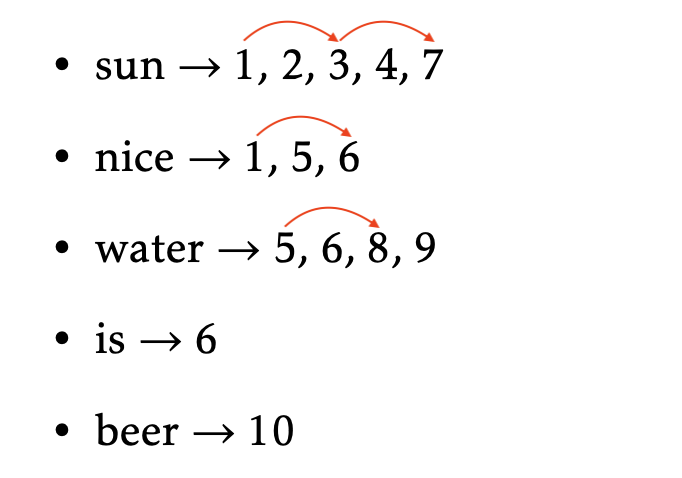
\includegraphics[width=0.8\textwidth]{img/skip_pointers.png}
  \end{center}
\end{figure}
Example query: \textbf{nice AND is}\\
\indent 1. Comparisons without skip pointers: 1 \& 6, 5 \& 6, 6 \& 6 $\Rightarrow$ 3 comparisons\\
\indent 2. Comparisons with skip pointers: 1 \& 6, 6 \& 6 $\Rightarrow$ 2 comparisons\\
\indent Without skip pointers we must compare the terms step by step, although 5 in \textbf{nice} is still smaller than 6 in \textbf{is}. With skip pointers we can skip the 5 in \textbf{nice} and directly go to the 6 in \textbf{nice}.\\

\clearpage
\section*{Pen and Paper Task 2}

\begin{lstlisting}
    tokenize(text: string):
        token = ''
        list_of_tokens = []

        for char in text:
            if char == ' ':  #whitespace
                list_of_tokens.add(token)
                token = '' #empty string
            if char is a symbol:
                list_of_tokens.add(token)
                list_of_token.add(char)
                token = '' #empty string
            else:
                token += char
                
        return list_of_tokens

\end{lstlisting}

\clearpage
\section*{Programming Task 1}
\lstinputlisting{code/script.py}
\end{document}